\documentclass{izpit}

\begin{document}

%==========================================================================
%               Sem vpisi podatke o izpitu
%==========================================================================
\FRACTIONSIMPLIFY{27}{1}{\skupnotock}{\nepomembno}%Sem vpiši (v polje trenutno {60}) skupno število točk, da paket naračuna kriterij ocenjevanj
\izpit[ucilnica = RAZRED, naloge = 6]%ucilnica RAZRED, lahko se sedezni red, ime in priimek, maturitetni
{Vektorji in potence ter koreni}{15. 1. 2024}{Čas pisanja je 45 minut.\\ Možno je doseči $\skupnotock$ točk.\\ Veliko uspeha!}
%==========================================================================
%               Nepomembno - Preskoči
%==========================================================================
\MAX{0.1}{0}{\tempepsilon}%shranimo epsilon... ne gre trik z ulomkom zato max
\MULTIPLY{\skupnotock}{0.89}{\odlicno}
\MULTIPLY{\skupnotock}{0.76}{\pravdobro}
\MULTIPLY{\skupnotock}{0.62}{\dobro}
\MULTIPLY{\skupnotock}{0.5}{\zadostno}
\ADD{\dobro}{\tempepsilon}{\dobroplus}
\ADD{\pravdobro}{\tempepsilon}{\pravdobroplus}
\ADD{\odlicno}{\tempepsilon}{\odlicnoplus}
\ROUND[1]{\dobroplus}{\dobroplus}
\ROUND[1]{\pravdobroplus}{\pravdobroplus}
\ROUND[1]{\odlicnoplus}{\odlicnoplus}
\ROUND[1]{\zadostno}{\zadostno}
\ROUND[1]{\dobro}{\dobro}
\ROUND[1]{\pravdobro}{\pravdobro}
\ROUND[1]{\odlicno}{\odlicno}\begin{small}
 \PlaceText{100mm}{33mm}{\begin{tabular}{ll}
    \multicolumn{2}{c}{\textbf{Kriterij ocenjevanja}} \\[0.5ex]
    Ocena & Tocke \\ \hline
    zadostno & $13 - 16$ \\
    dobro & $17 - 20$ \\
    prav dobro & $21 - 23$ \\
    odlicno & $24$--
  \end{tabular}}\end{small}
 \ifthenelse{\boolean{@maturitetni}}{\newpage}%TO JE ZELO GRDA KODA a ker ne gre kriterij v class ni druge moznosti
%==========================================================================
%               Sem vpisi naloge
%   za dodatek koordinatnega sistema daj pod navodila naloge \dodatek{\[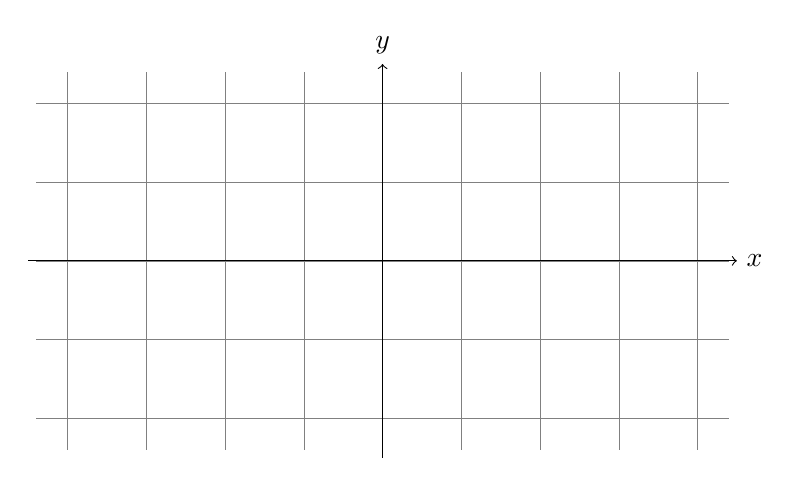
\begin{tikzpicture}
        \draw[help lines,step=1cm] (-4.4,-2.4) grid (4.4,2.4);
        \draw[->] (-4.5,0) -- (4.5,0) node[right] {$x$};
        \draw[->] (0,-2.5) -- (0,2.5) node[above] {$y$};
\end{tikzpicture}\]}
%   oz. za kompleksno ravnino \dodatek\[\begin{tikzpicture}
        \draw[help lines,step=1cm] (-4.4,-2.4) grid (4.4,2.4);
        \draw[->] (-4.5,0) -- (4.5,0) node[right] {$Re$};
        \draw[->] (0,-2.5) -- (0,2.5) node[above] {$Im$};
\end{tikzpicture}\]
%==========================================================================

\naloga[\tocke{5}]
  Dan je paralelogram $ABCD$. Točka $M$ je razpolovišče daljice $BC$, točka $N$ pa leži na daljici $AD$, da velja $|AN|:|AD|=2:5$. V kolikšnem razmerju deli daljica $MD$ daljico $NC$.



\naloga[\tocke{4}]
  V ravnini sta dani točki $X=(1,1)$ in $Y=(3,-4)$.
  \podnaloga[1] Določi koordinate vektorja $\vec{a}=\vec{XY}$.
  \prostor[1]
  \podnaloga[3]
  Določi parameter $m$, da bosta vektorja $\vec{a}=(2,-3)$ in $\vec{b}=(m+2,-1)$, kjer je  kolinearna.
  \prostor[1]
  
\naloga*[\tocke{5}]
  Dolžina vektorja $\vec{a}-\vec{b}$ je 3, dolžina vektorja $\vec{b}$ je 2, dolžina $\vec{a}$ pa 1. Natančno izračunaj kot med vektorjema $\vec{a}$ in $\vec{b}$.
  \prostor[2]

\naloga[\tocke{4}]
  Poenostavi%445g
  \[\sqrt[40]{x^{25}y^{15}}-2\cdot \sqrt[8]{x^{10}y^{2}}\cdot\sqrt[8]{x^{-5}y}+\sqrt[4]{x\sqrt{x^3 y^3}}.\]
  \prostor[1]


\naloga*[\tocke{4}]%459i
  Poenostavi
  \[\frac{\left(a^{-\frac{2}{3}}b^{\frac{1}{9}}\right)^{-2}\cdot\left(a^0 +3\right)^{-\frac{1}{2}}}{\sqrt[3]{a^2 b}}.\]
  \prostor[1]

\naloga[\tocke{5}]
  Reši enačbo
  \[\sqrt[3]{31-x+\sqrt{x-2}}=3.\]

\end{document}